% \section{Análisis del proceso actual}
% A continuación se describe el proceso para reportar incidentes por parte de los ciudadanos a través del servicio
% de emergencia Ecu 911. Este proceso se basa en la información obtenida de la entrevista realizada al teniente
% coronel de estado mayor Christian Iván Quintana Guerra, En la Figura 1 se detalla el siguiente proceso, donde:

% \begin{enumerate}
%     \item El usuario llama al número de emergencia del ECU 911.
%     \item El operador recibe la llamada y solicita la información necesaria al usuario.
%     \item En base al tipo de incidente, el operador asigna la emergencia a la entidad correspondiente.
%     \item La entidad correspondiente recibe la emergencia y envía una unidad al lugar del incidente.
%     \item La unidad llega al lugar del incidente, donde:
%           \begin{enumerate}
%               \item La unidad verifica la información con la que cuenta:
%                     \begin{enumerate}
%                         \item Si cuenta con la información necesaria, la emergencia es atendida.
%                         \item Si no cuenta con la información necesaria, se solicita a la víctima o testigo la información faltante.
%                     \end{enumerate}
%           \end{enumerate}
%     \item Se reporta el incidente la atención de la emergencia y la información es almacenada en una matriz de excel.
% \end{enumerate}

% \begin{figure}[H]
%     \centering
%     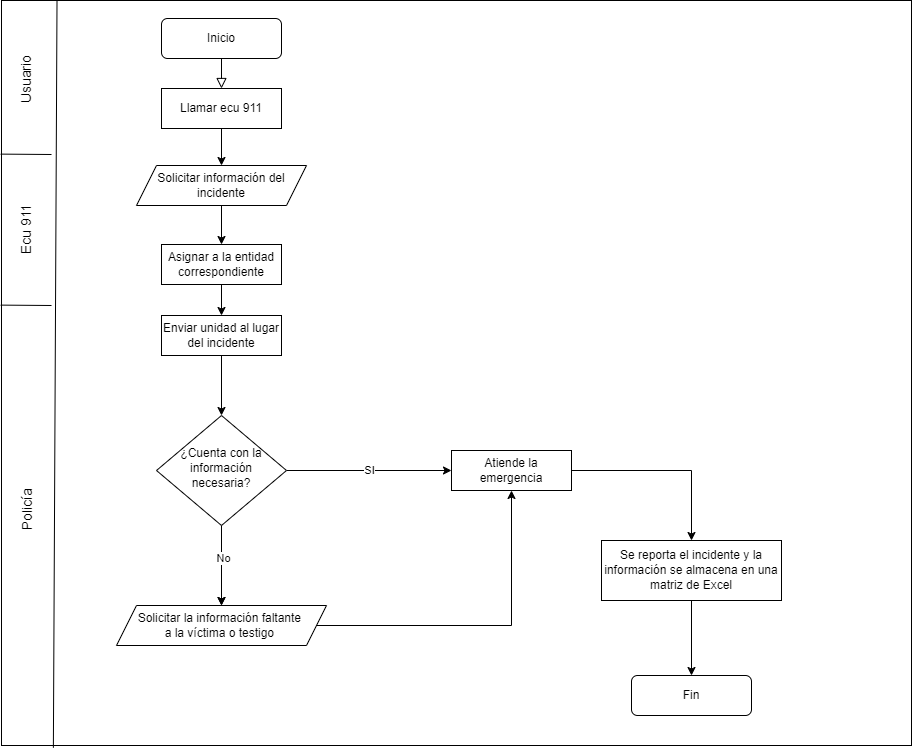
\includegraphics[width=0.8\textwidth]{chapters/III-resultados-y-discusion/resources/images/proceso-actual.png}
%     \caption{Proceso actual de reporte de incidentes al ECU 911.}
%     \label{fig:proceso-actual}
% \end{figure}

\section{Análisis de procesos}

\subsubsection{Análisis del proceso propuesto}

En la Figura \ref{fig:proceso-propuesto} se presenta el proceso propuesto para él envió de alertas de emergencia con
ubicación en tiempo real, en donde:

\begin{enumerate}
    \item Si el usuario no se encuentra registrado en el sistema:
          \begin{enumerate}
              \item El usuario se registra en el sistema.
              \item El usuario inicia sesión en el sistema.
          \end{enumerate}
    \item El usuario ingresa miembros a su grupo familiar.
    \item El usuario selecciona un tipo de incidente.
          % \item El usuario envía la alerta de emergencia presionando el bot��������n de pánico durante 3 segundos.
    \item El usuario envía la alerta de emergencia presionando el botón de pánico durante 3 segundos.
    \item Se envía una notificación a los miembros del grupo familiar del usuario y los policías dentro de la zona de emergencia junto con la ubicación en tiempo real.
    \item El Ecu 911 recibe la alerta de emergencia y la asigna a la entidad correspondiente.
    \item Si el tipo de incidente no es el correcto:
          \begin{enumerate}
              \item Ingresar la información correcta sobre el incidente.
              \item La emergencia es atendida.
          \end{enumerate}
\end{enumerate}

\begin{figure}[H]
    \centering
    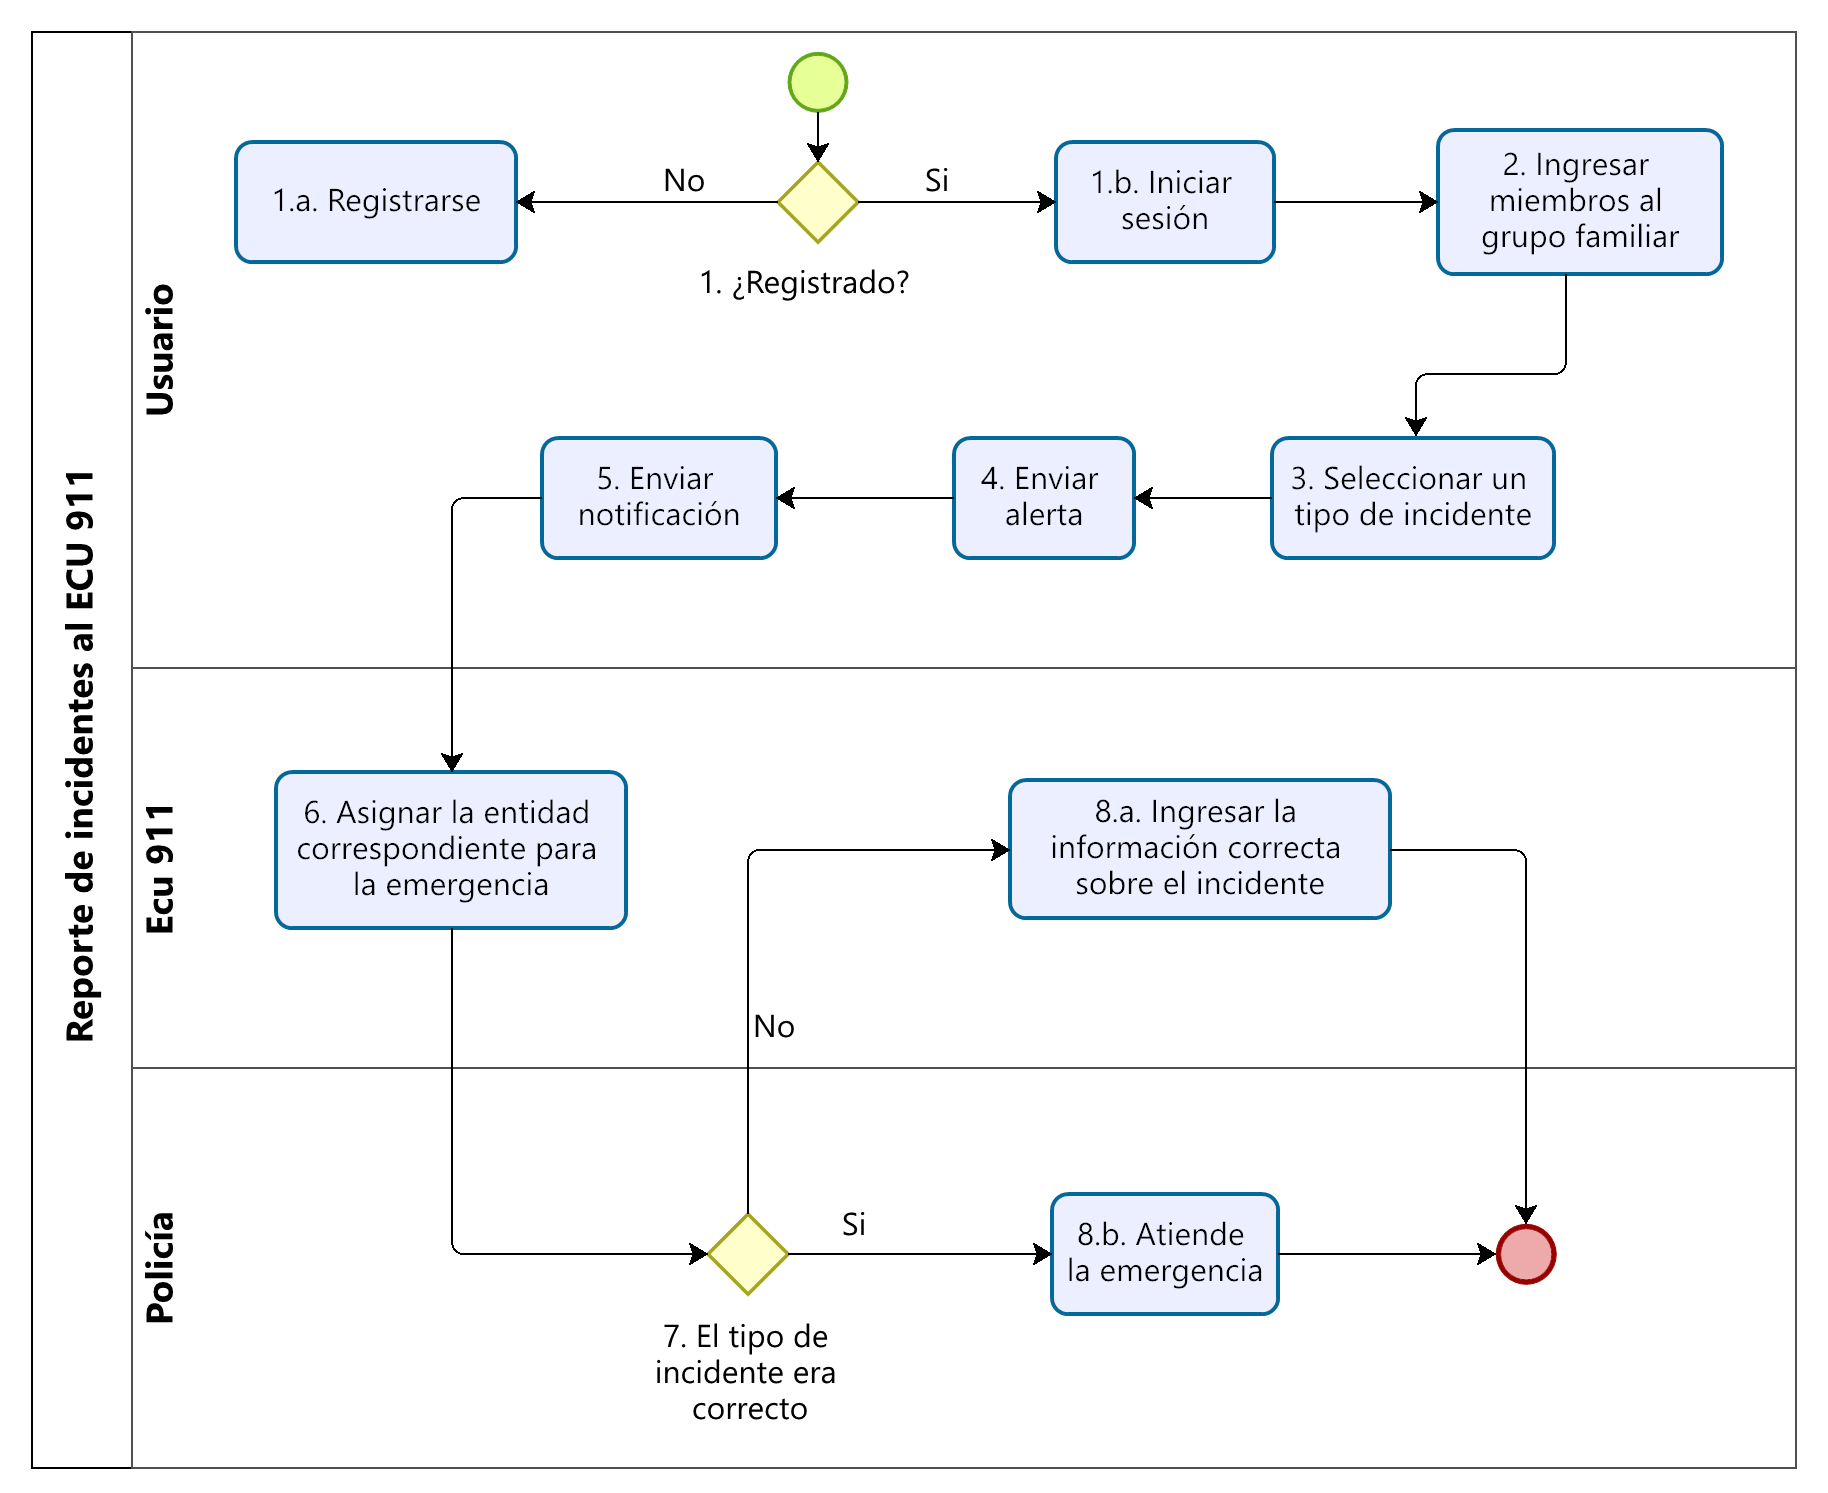
\includegraphics[width=1\textwidth]{chapters/III-resultados-y-discusion/resources/images/proceso-propuesto.png}
    \caption{Proceso propuesto de reporte de incidentes al ECU 911.}
    \label{fig:proceso-propuesto}
\end{figure}

\subsubsection{Análisis del proceso de BI}

En la Figura \ref{fig:proceso-bi} se presenta el proceso de Business Intelligence (BI) propuesto para el análisis de los incidentes reportados al ECU 911, en donde:

\begin{enumerate}
    \item Se seleccionan las preguntas del negocio.
    \item Se identifica los indicadores y perspectivas.
    \item Se declara el grano.
    \item Se identifica las dimensiones y atributos.
    \item Se crea el esquema dimensional.
    \item Se realiza el proceso ETL.
    \item Se crea el cubo OLAP.
    \item Se visualiza los datos mediante gráficos y reportes.
\end{enumerate}

\begin{figure}[H]
    \centering
    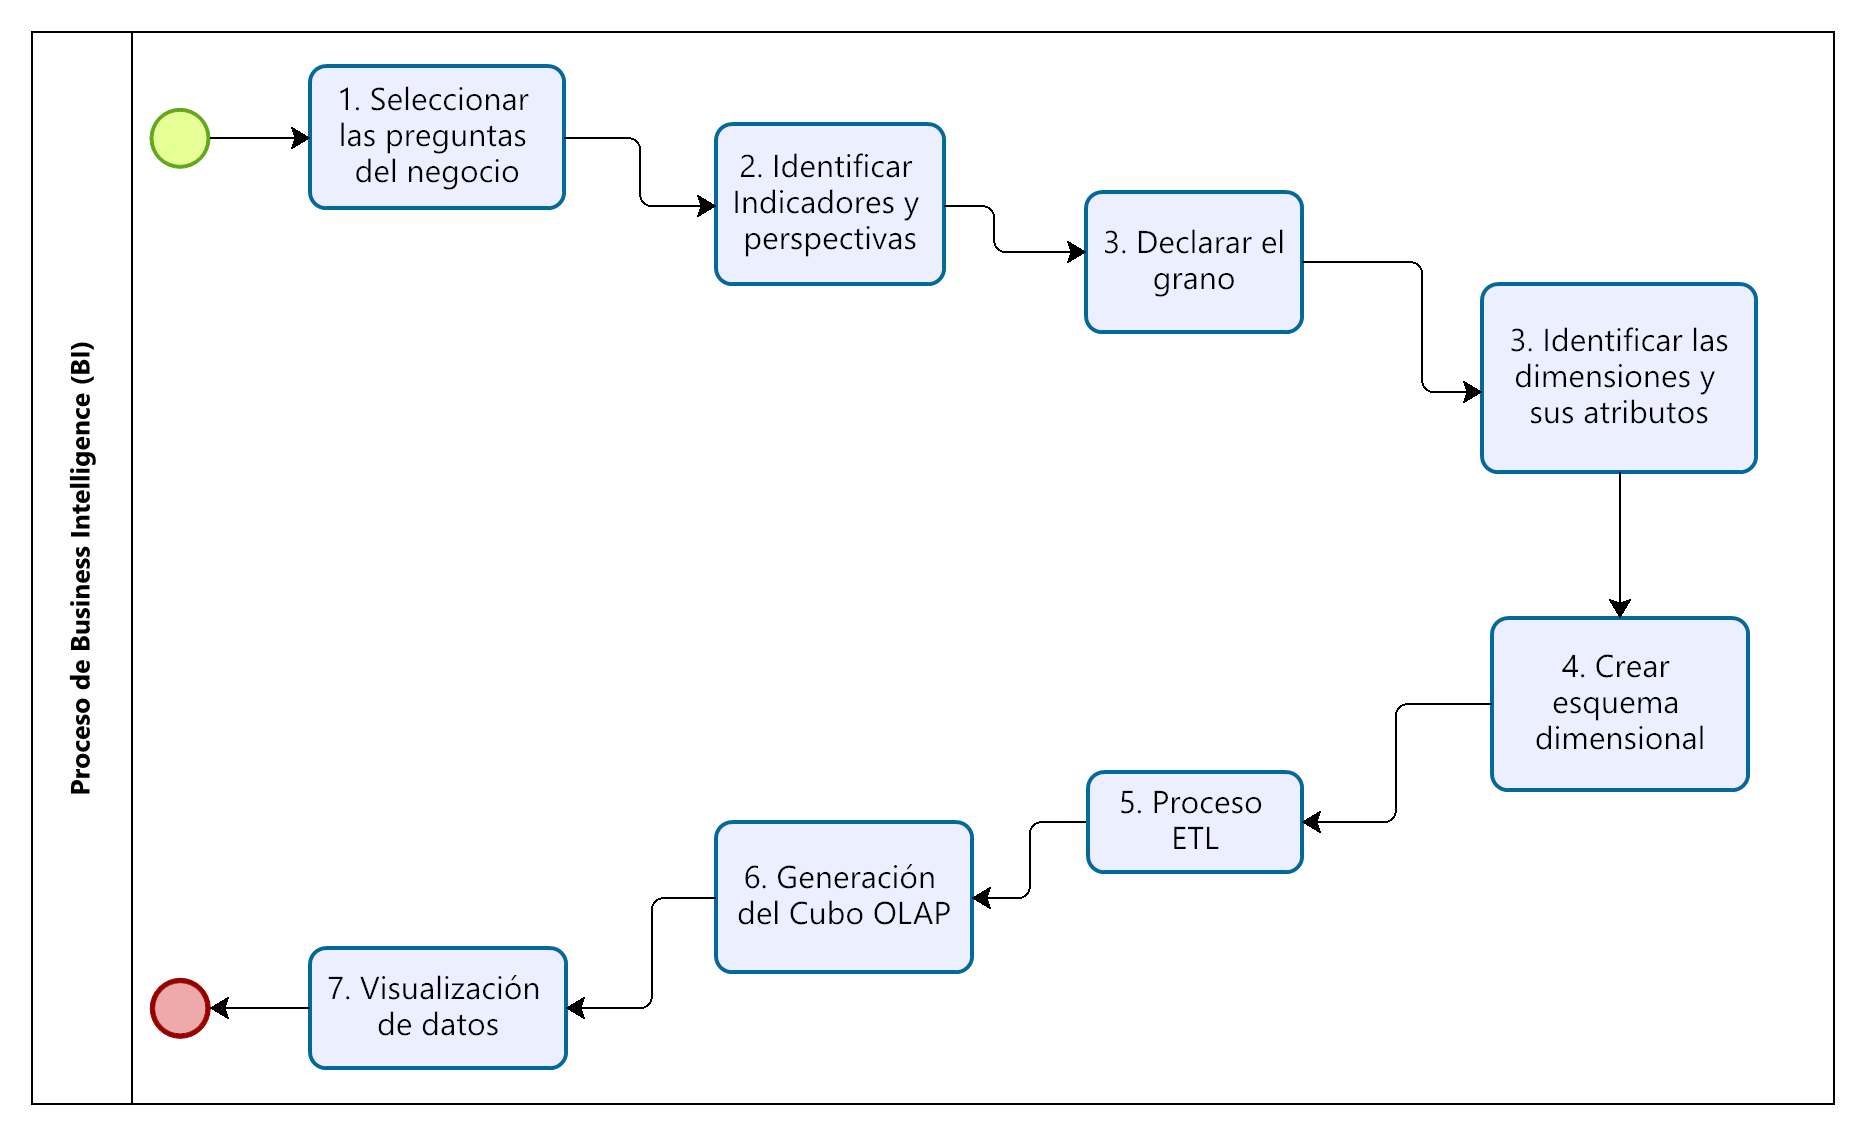
\includegraphics[width=1\textwidth]{chapters/III-resultados-y-discusion/resources/images/proceso-bi.png}
    \caption{Proceso de Business Intelligence (BI) para el análisis de incidentes reportados al ECU 911.}
    \label{fig:proceso-bi}
\end{figure}